\documentclass{article}

\usepackage[papersize={20cm,30cm},left=0cm,right=0cm,top=0cm,bottom=0cm]{geometry}
\usepackage{tikz}              % zum Zeichnen von Abbildungen etc.
\usetikzlibrary{backgrounds,mindmap}

\definecolor{f1}{HTML}{7FA0A0}
\definecolor{f2}{HTML}{1133FF}
\definecolor{f3}{HTML}{36648B}
\definecolor{f7}{HTML}{5692B4}
\definecolor{f5}{HTML}{78BCEE}
\definecolor{f6}{HTML}{00FFFF}
\definecolor{f9}{HTML}{00DD99}
\definecolor{f8}{HTML}{FFFFA6}
\definecolor{f4}{HTML}{00CC66}
\definecolor{f10}{HTML}{00BB22}
\definecolor{darkgreen}{HTML}{006600}
\definecolor{scipyellow}{HTML}{FFFFE6}

\pagestyle{empty}

\begin{document}

\centering
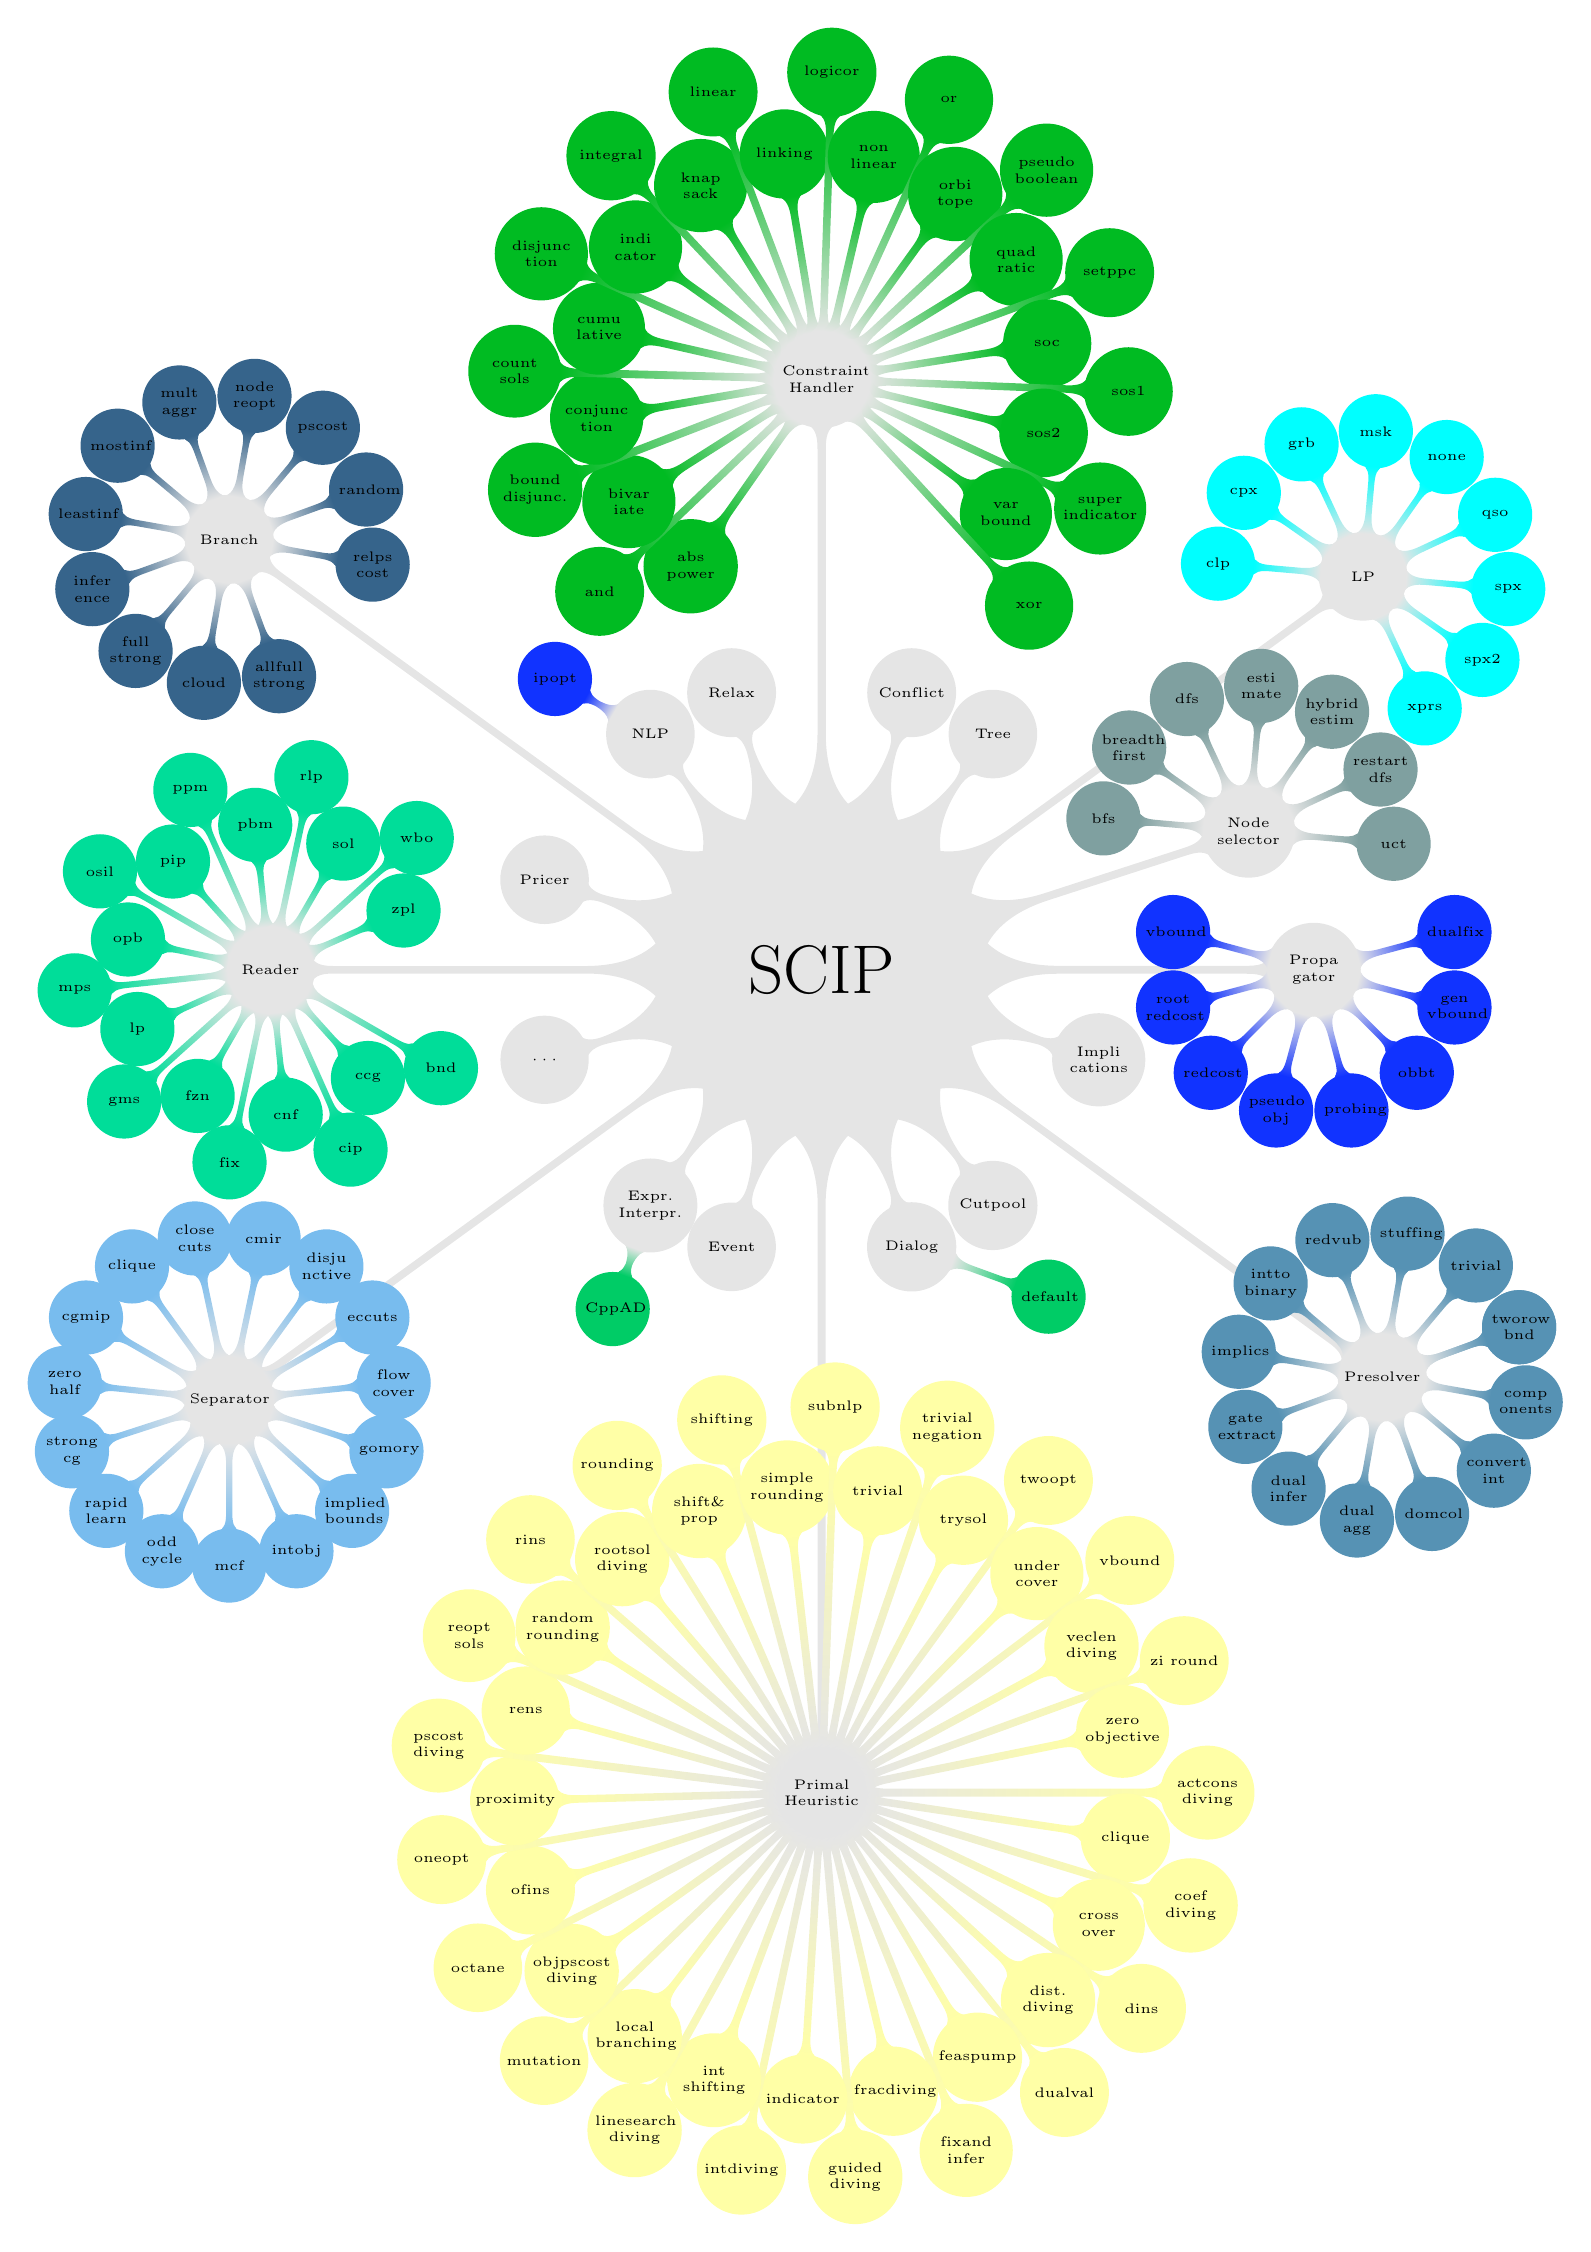
\begin{tikzpicture}[mindmap,concept color=gray!20]
  \tikzstyle{root concept} = [concept, text width=1cm, minimum size=1cm, sibling angle=18];
  \tikzstyle{level 1 concept} = [level 3 concept,level distance=3.7cm,sibling angle=18, minimum size=.7cm];
  \tikzstyle{level 2 concept} = [level 4 concept];%sibling angle=18, minimum size=1cm, text width=1cm];
  \tikzstyle{branchconcept} = [level 2 concept,concept color=f3];
  \tikzstyle{conshdlrconcept} = [level 1 concept,sibling angle=25,concept color=f10,minimum size=.6cm];
  \tikzstyle{conshdlrconceptodd} = [conshdlrconcept, sibling angle=11.3, level distance=3.9cm];
  \tikzstyle{conshdlrconcepteven} = [conshdlrconceptodd, level distance=2.9cm];
  \tikzstyle{lpiconcept} = [level 2 concept,concept color=f6];
  \tikzstyle{dialogconcept} = [level 2 concept,concept color=f4];
  \tikzstyle{displayconcept} = [level 2 concept,concept color=f4];
  \tikzstyle{nodeselectionconcept} = [level 2 concept,sibling angle=30,concept color=f1];
  \tikzstyle{presolverconcept} = [level 2 concept,concept color=f7];
  %\tikzstyle{presolverconcepteven} = [presolverconceptodd];%, level distance=2.5cm];
  \tikzstyle{heurconcepteven} = [level 1 concept, sibling angle=8.5, level distance=4.9cm, concept color=f8, minimum size=.7cm];
  \tikzstyle{heurconceptodd} = [heurconcepteven, level distance=3.9cm, minimum size=.7cm];
  \tikzstyle{readerconceptodd} = [level 2 concept,sibling angle=18,concept color=f9];
  \tikzstyle{readerconcepteven} = [readerconceptodd, level distance=2.5cm];
  \tikzstyle{sepaconcept} = [level 2 concept,sibling angle=24, level distance=2.1cm,concept color=f5];
  \tikzstyle{propconcept} = [level 2 concept,sibling angle=30,concept color=f2];
  \tikzstyle{eventconcept} = [level 2 concept,concept color=f4];
  \tikzstyle{nlpiconcept} = [level 2 concept, level distance=1.4cm,concept color=f2];
  \tikzstyle{exprintconcept} = [level 2 concept, level distance=1.4cm,concept color=f4];

  \node [concept] {\Huge SCIP}
  [clockwise from=-90]
  child[level distance=10.45cm] { node[concept, minimum size=1cm] (Heuristic) {Primal\\Heuristic}
    [clockwise from=0]
    child[heurconcepteven] { node[concept] (actconsdiving) {actcons\\diving}}
    child[heurconceptodd]  { node[concept] (clique) {clique}}
    child[heurconcepteven]  { node[concept] (coefdiving) {coef\\diving}}
    child[heurconceptodd] { node[concept] (crossover) {cross\\over}}
    child[heurconcepteven]  { node[concept] (dins) {dins}}
    child[heurconceptodd]  { node[concept] (distribdiving) {dist.\\diving}}
    child[heurconcepteven] { node[concept] (dualval) {dualval}}
    child[heurconceptodd]  { node[concept] (feaspump) {feaspump}}
    child[heurconcepteven] { node[concept] (fixandinfer) {fixand\\infer}}
    child[heurconceptodd]  { node[concept] (fracdiving) {fracdiving}}
    child[heurconcepteven] { node[concept] (guideddiving) {guided\\diving}}
    child[heurconceptodd]   { node[concept] (indicator) {indicator}}
    child[heurconcepteven]  { node[concept] (intdiving) {intdiving}}
    child[heurconceptodd]   { node[concept] (intshifting) {int\\shifting}}
    child[heurconcepteven]  { node[concept] (linesearchdiving) {linesearch\\diving}}
    child[heurconceptodd]   { node[concept] (localbranching) {local\\branching}}
    child[heurconcepteven]  { node[concept] (mutation) {mutation}}
    child[heurconceptodd]  { node[concept] (objpscostdiving) {objpscost\\diving}}
    child[heurconcepteven]   { node[concept] (octane) {octane}}
    child[heurconceptodd]  { node[concept] (ofins) {ofins}}
    child[heurconcepteven] { node[concept] (oneopt) {oneopt}}
    child[heurconceptodd]   { node[concept] (proximity) {proximity}}
    child[heurconcepteven]  { node[concept] (pscostdiving) {pscost\\diving}}
    child[heurconceptodd]   { node[concept] (rens) {rens}}
    child[heurconcepteven]  { node[concept] (reoptsols) {reopt\\sols}}
    child[heurconceptodd]  { node[concept] (randround) {random\\rounding}}
    child[heurconcepteven]   { node[concept] (rins) {rins}}
    child[heurconceptodd]  { node[concept] (rootsoldiving) {rootsol\\diving}}
    child[heurconcepteven]   { node[concept] (rounding) {rounding}}
    child[heurconceptodd]  { node[concept] (shiftandpropagate) {shift\&\\prop}}
    child[heurconcepteven]  { node[concept] (shifting) {shifting}}
    child[heurconceptodd]   { node[concept] (simplerounding) {simple\\rounding}}
    child[heurconcepteven]   { node[concept] (subnlp) {subnlp}}
    child[heurconceptodd]  { node[concept] (trivial) {trivial}}
    child[heurconcepteven]  { node[concept] (trivialnegation) {trivial\\negation}}
    child[heurconceptodd]    { node[concept] (trysol) {trysol}}
    child[heurconcepteven]  { node[concept] (twoopt) {twoopt}}
    child[heurconceptodd]    { node[concept] (undercover) {under\\cover}}
    child[heurconcepteven] { node[concept] (vbounds) {vbound}}
    child[heurconceptodd]   { node[concept] (veclendiving) {veclen\\diving}}
    child[heurconcepteven] { node[concept] (ziround) {zi round}}
    child[heurconceptodd]  { node[concept] (zeroobj) {zero\\objective}}
    }
%   child { node[concept] (Variable) {Variable}}
  child { node[concept] (Event) {Event}}
   child { node[concept] (Exprint) {Expr. Interpr.}
     [clockwise from=-110]
     child[exprintconcept] { node[concept] (cppad) {CppAD}}
   }
  child[level distance=9.3cm] { node[concept] (Separator) {Separator}
    [clockwise from=150]
    child[sepaconcept] { node[concept] (cgmip) {cgmip}}
    child[sepaconcept] { node[concept] (clique) {clique}}
    child[sepaconcept] { node[concept] (closecuts) {close\\cuts}}
    child[sepaconcept] { node[concept] (cmir) {cmir}}
    child[sepaconcept] { node[concept] (disjunctive) {disju\\nctive}}
    child[sepaconcept] { node[concept] (eccuts) {eccuts}}
    child[sepaconcept] { node[concept] (flowcover) {flow\\cover}}
    child[sepaconcept] { node[concept] (gomory) {gomory}}
    child[sepaconcept] { node[concept] (impliedbounds) {implied\\bounds}}
    child[sepaconcept] { node[concept] (intobj) {intobj}}
    child[sepaconcept] { node[concept] (mcf) {mcf}}
    child[sepaconcept] { node[concept] (oddcycle) {odd\\cycle}}
    child[sepaconcept] { node[concept] (rapidlearning) {rapid\\learn}}
    child[sepaconcept] { node[concept] (strongcg) {strong\\cg}}
    child[sepaconcept] { node[concept] (zerohalf) {zero\\half}}
  }
  child { node[concept] (dots) {$\cdots$}}
  child[level distance=7.0cm] { node[concept] (Reader) {Reader}
    [clockwise from=-30]
    child[readerconcepteven] { node[concept] (bnd) {bnd}}
    child[readerconceptodd] { node[concept] (ccg) {ccg}}
    child[readerconcepteven] { node[concept] (cip) {cip}}
    child[readerconceptodd] { node[concept] (cnf) {cnf}}
    child[readerconcepteven] { node[concept] (fix) {fix}}
    child[readerconceptodd] { node[concept] (fzn) {fzn}}
    child[readerconcepteven] { node[concept] (gms) {gms}}
    child[readerconceptodd] { node[concept] (lp) {lp}}
    child[readerconcepteven] { node[concept] (mps) {mps}}
    child[readerconceptodd] { node[concept] (opb) {opb}}
    child[readerconcepteven] { node[concept] (osil) {osil}}
    child[readerconceptodd] { node[concept] (pip) {pip}}
    child[readerconcepteven] { node[concept] (ppm) {ppm}}
    child[readerconceptodd] { node[concept] (pbm) {pbm}}
    child[readerconcepteven] { node[concept] (rlp) {rlp}}
    child[readerconceptodd] { node[concept] (sol) {sol}}
    child[readerconcepteven] { node[concept] (wbo) {wbo}}
    child[readerconceptodd] { node[concept] (zpl) {zpl}}
  }
  child { node[concept] (Pricer) {Pricer}}
  child[level distance=9.3cm] { node[concept] (Branch) {Branch}
    [clockwise from=-70]
    child[branchconcept] { node[concept] (allfullstring) {allfull\\strong}}
    child[branchconcept] { node[concept] (cloud) {cloud}}
    child[branchconcept] { node[concept] (fullstrong) {full\\strong}}
    child[branchconcept] { node[concept] (inference) {infer\\ence}}
    child[branchconcept] { node[concept] (leastinf) {leastinf}}
    child[branchconcept] { node[concept] (mostinf) {mostinf}}
    child[branchconcept] { node[concept] (multaggr) {mult\\aggr}}
    child[branchconcept] { node[concept] (nodereopt) {node\\reopt}}
    child[branchconcept] { node[concept] (pscost) {pscost}}
    child[branchconcept] { node[concept] (random) {random}}
    child[branchconcept] { node[concept] (relpscost) {relps\\cost}}
  }
%   child { node[concept] (Display) {Display}
%     [clockwise from=-155]
%     child[displayconcept] { node[concept] (default) {default}}
%   }
  child { node[concept] (NLP) {NLP}
    [clockwise from=150]
    child[nlpiconcept] { node[concept] (ipopt) {ipopt}}
  }
  child { node[concept] (Relaxer) {Relax}}
  child[level distance=7.5cm,minimum size=1.2cm] { node[concept] (ConsHdlr) {Constraint\\Handler}
    [clockwise from=-125]
    child[conshdlrconcepteven] { node[concept] (abspower) {abs\\power}}
    child[conshdlrconceptodd] { node[concept] (and) {and}}
    child[conshdlrconcepteven] { node[concept] (bivariate) {bivar\\iate}}
    child[conshdlrconceptodd] { node[concept] (bounddisjunction) {bound\\disjunc.}}
    child[conshdlrconcepteven] { node[concept] (conjunction) {conjunc\\tion}}
    child[conshdlrconceptodd] { node[concept] (countsols) {count\\sols}}
    child[conshdlrconcepteven] { node[concept] (cumulative) {cumu\\lative}}
    child[conshdlrconceptodd] { node[concept] (disjunction) {disjunc\\tion}}
    child[conshdlrconcepteven] { node[concept] (indicator) {indi\\cator}}
    child[conshdlrconceptodd] { node[concept] (integral) {integral}}
    child[conshdlrconcepteven] { node[concept] (knapsack) {knap\\sack}}
    child[conshdlrconceptodd] { node[concept] (linear) {linear}}
    child[conshdlrconcepteven] { node[concept] (linking) {linking}}
    child[conshdlrconceptodd] { node[concept] (logicor) {logicor}}
    child[conshdlrconcepteven] { node[concept] (nonlinear) {non\\linear}}
    child[conshdlrconceptodd] { node[concept] (or) {or}}
    child[conshdlrconcepteven] { node[concept] (orbitope) {orbi\\tope}}
    child[conshdlrconceptodd] { node[concept] (pseudoboolean) {pseudo\\boolean}}
    child[conshdlrconcepteven] { node[concept] (quadratic) {quad\\ratic}}
    child[conshdlrconceptodd] { node[concept] (setppc) {setppc}}
    child[conshdlrconcepteven] { node[concept] (soc) {soc}}
    child[conshdlrconceptodd] { node[concept] (sos1) {sos1}}
    child[conshdlrconcepteven] { node[concept] (sos2) {sos2}}
    child[conshdlrconceptodd] { node[concept] (superindicator) {super\\indicator}}
    child[conshdlrconcepteven] { node[concept] (varbound) {var\\bound}}
    child[conshdlrconceptodd] { node[concept] (xor) {xor}}
  }
  child { node[concept] (Conflict) {Conflict}}
  child { node[concept] (Tree) {Tree}}
  child[level distance=8.5cm] { node[concept] (LP) {LP}
    [clockwise from=175]
    child[lpiconcept] { node[concept] (clp) {clp}}
    child[lpiconcept] { node[concept] (cpx) {cpx}}
    child[lpiconcept] { node[concept] (grb) {grb}}
    child[lpiconcept] { node[concept] (msk) {msk}}
    child[lpiconcept] { node[concept] (none) {none}}
    child[lpiconcept] { node[concept] (qso) {qso}}
    child[lpiconcept] { node[concept] (spx) {spx}}
    child[lpiconcept] { node[concept] (spx2) {spx2}}
    child[lpiconcept] { node[concept] (xprs) {xprs}}
  }
  child[level distance=5.7cm] { node[concept] (Nodeselector) {Node\\selector}
    [clockwise from=175]
    child[nodeselectionconcept] { node[concept] (bfs) {bfs}}
    child[nodeselectionconcept] { node[concept] (breadth) {breadth\\first}}
    child[nodeselectionconcept] { node[concept] (dfs) {dfs}}
    child[nodeselectionconcept] { node[concept] (estimate) {esti\\mate}}
    child[nodeselectionconcept] { node[concept] (hybridestim) {hybrid\\estim}}
    child[nodeselectionconcept] { node[concept] (restartdfs) {restart\\dfs}}
    child[nodeselectionconcept] { node[concept] (uct) {uct}}
  }
  child[level distance=6.25cm] { node[concept] (Propagator) {Propa\\gator}
    [clockwise from=15]
    child[propconcept] { node[concept] (dualfix) {dualfix}}
    child[propconcept] { node[concept] (genvbounds) {gen\\vbound}}
    child[propconcept] { node[concept] (obbt) {obbt}}
    child[propconcept] { node[concept] (probing) {probing}}
    child[propconcept] { node[concept] (pseudoobj) {pseudo\\obj}}
    child[propconcept] { node[concept] (redcost) {redcost}}
    child[propconcept] { node[concept] (rootredcost) {root\\redcost}}
    child[propconcept] { node[concept] (vbounds) {vbound}}
  }
  child { node[concept] (Implications) {Impli\\cations}}
  child[level distance=8.8cm] { node[concept] (Presolver) {Presolver}
    [clockwise from=20]
    child[presolverconcept] { node[concept] (boundshift) {bound\\shift}}
    child[presolverconcept] { node[concept] (components) {comp\\onents}}
    child[presolverconcept] { node[concept] (convertinttobinary) {convert\\int}}
    child[presolverconcept] { node[concept] (domcol) {domcol}}
    child[presolverconcept] { node[concept] (dualagg) {dual\\agg}}
    child[presolverconcept] { node[concept] (dualinfer) {dual\\infer}}
    child[presolverconcept] { node[concept] (gateextract) {gate\\extract}}
    child[presolverconcept] { node[concept] (implics) {implics}}
    child[presolverconcept] { node[concept] (inttobinary) {intto\\binary}}
    child[presolverconcept] { node[concept] (redvub) {redvub}}
    child[presolverconcept] { node[concept] (redvub) {stuffing}}
    child[presolverconcept] { node[concept] (trivial) {trivial}}
    child[presolverconcept] { node[concept] (tworowbnd) {tworow\\bnd}}
  }
  child { node[concept] (Cutpool) {Cutpool}}
  child { node[concept] (Dialog) {Dialog}
    [clockwise from=-20]
    child[dialogconcept] { node[concept] (default) {default}}
  }
;
\end{tikzpicture}

\end{document}
